\section{Theoretische Grundlagen}
Operationsverstärker sind elektrische Bauteile aus dem Bereich der analogen
Signalverarbeitung und bestehen aus Schaltungen von Transistoren. Bei der
Planung von Schaltungen mit Operationsverstärkern werden diese als idealisierte
Bauteile, sogenannte ideale Operationsverstärker, betrachtet. Tatsächlich
weichen reale Operationsverstärker in ihren Eigenschaften vom idealisierten
Bauteil ab, allerdings nicht soweit, als dass eine ideale Beschreibung nicht
gerechtfertigt wäre. \\
\noindent Verschiedene Beschaltungen führen bei einem Operationsverstärker zu
verschiedenen Funktionsweisen wie beispielsweise Gegenkopplung oder
Mitkopplung. Die Funktionsprinzipien dieser Schaltungen werden für exemplarische
Schaltungen erläutert.
\subsection{Eigenschaften idealer Operationsverstärker}
Ideale Operationsverstärker kennzeichnen sich dadurch aus, dass ihre
Leerlaufverstärkung $\frac{U_A}{U_E}$ als unendlich groß angenommen wird und
dass kein Strom in den Operationsverstärker hineinfließen kann, da sein
Eingangswiderstand unendlich groß ist. Ferner verschwindet der
Ausgangswiderstand eines Operationsverstärkers und seine Übertragungsbandbreite
umfasst einen unendlich großen Frequenzbereich, ohne dass eine Phasendrehung
stattfindet \cite{federau}. \\
\noindent Operationsverstärker sind Differenzverstärker. Ihre Ausgangsspannung $U_A$
ist proportional zur Differenz zwischen der Eingangsspannung $U_P$ am
nicht-invertierenden Eingang und der Eingangsspannung $U_N$ am
invertierenden Eingang. Der Proportionalitätsfaktor sei $V$. Damit gilt
\begin{align}
  U_A = V \cdot \left(U_P - U_N \right).
  \label{eqn:01}
\end{align}
\noindent Der Verstärkungsfaktor liegt typischerweise in einer Größenordnung
zwischen $\num{e4}$ und $\num{e5}$, sofern die Versorgungsspannung $U_V$ im
zulässigen Spannungsintervall (bauartbedingt) liegt. Aufgrund der hohen
Verstärkung liegt die Spannungsdifferenz zwischen $U_P$ und $U_N$ meist im
Bereich einiger Millivolt, eine höhere Spannungsdifferenz führt dann nicht
zu größeren Verstärkungen, sondern die Verstärkung durch den Operationsverstärker
geht in einen Bereich der Sättigung, wie in \autoref{fig:01} dargestellt \cite{hs-fulda}.
\begin{figure}
  \centering
  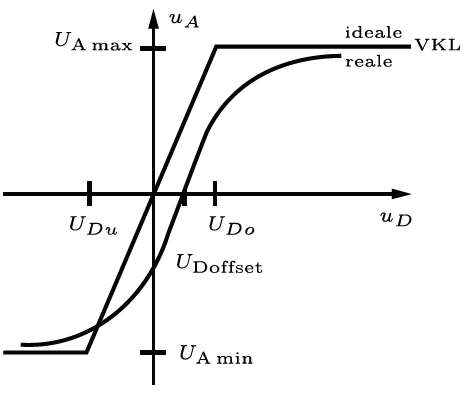
\includegraphics[scale=0.5]{ressources/figure_01.png}
  \caption{Verstärkungskennlinie für idealen und realen Operationsverstärker. $U_\text{Doffset}$
  kennzeichnet die Eingangs-Offsetspannung, $U_\text{Du}$ und $U_\text{Do}$ kennzeichnen
  die untere und obere Grenze des linearen Verstärkungsbereichs \cite{elektrotechnik}.}
  \label{fig:01}
\end{figure}
\noindent Die Aussteuergrenze (Sättigungsbereich) liegt etwa $\SI{1}{\volt}$
unterhalb der Betriebsspannung $U_B$ des Operationsverstärkers \cite{federau}, der
lineare Bereich damit zwischen
\begin{align}
  - U_B < U_A < + U_B,
  \label{eqn:02}
\end{align}
\noindent wobei die Ausgangsspannung $U_A$ nicht derjenigen in \autoref{fig:01}
entspricht. \\
\newline
\noindent Das Schaltsymbol eines Operationsverstärkers ist in \autoref{fig:02}
dargestellt. Wenngleich ein Operationsverstärker eine Vielzahl an
Anschlusskontakten besitzt, sind im Schaltzeichen lediglich der
invertierende Eingang $(-)$, der nicht-invertierende Eingang $(+)$ sowie der
Ausgang gekennzeichnet.
\begin{figure}
  \centering
  \includegraphics[scale=0.5]{ressources/figure_2.png}
  \caption{Schaltzeichen eines Operationsverstärkers \cite{federau}.}
  \label{fig:02}
\end{figure}
\subsection{Reale Operationsverstärker}
\noindent Bevor die Funktionsweisen der Gegen- und Mitkopplung am Beispiel
verschiedener Schaltungen erläutert werden, wird ein realer Operationsverstärker
betrachtet. Anders als ideale Operationsverstärker besitzen reale
Operationsverstärker eine endliche Leerlaufverstärkung und endliche
Eingangswiderstände. In Abhängigkeit vom jeweiligen Typ ist der Ausgangswiderstand
größer Null \cite{federau}.\\
\noindent Während beim idealen Operationsverstärker keine Gleichtaktverstärkung
auftritt, berechnet sich diese beim realen Operationsverstärker mithilfe der
Formel
\begin{align}
  V_\text{Gl} = \frac{U_a}{U_\text{Gl}} \qquad \text{mit} \qquad U_\text{Gl} = \frac{U_P + U_N}{2}.
  \label{eqn:03}
\end{align}
\noindent Ist die Gleichtaktverstärkung bekannt, so lässt sich die Offsetspannung
ermitteln. $U_\text{Gl}$ wird dabei so gewählt, dass $U_A \approx 0$ ist. Wird
zusätzlich die Annahme $\bigr| \frac{1}{2} \cdot U_0 \bigr| << \bigr| U_\text{Gl} \bigr|$
getroffen, gilt die Relation
\begin{align}
  0 &= V_\text{Gl} \cdot U_\text{Gl} - V_0 \cdot U_0 \\
  \implies U_0 &= \frac{V_\text{Gl}}{V_0} \cdot U_\text{Gl},
  \label{eqn:04}
\end{align}
\noindent wobei $V_0 = - \frac{U_A}{U_N}$ \cite{muenster}.
\subsection{Operationsverstärker in Schaltungen}
Einfache Rechenoperationen und die Steuerung von Signalen lassen sich durch
Schaltungen mit Widerständen und Kondensatoren realisieren.
\subsubsection{Invertierender Linearverstärker}
Ein invertierender Linearverstärker arbeitet mit einer Gegenkopplung, welche
sicherstellen soll, dass die Verstärkung unverzerrt ist. Dies wird durch eine
Rückführung des Ausgangssignals auf den Signaleingang erreicht. \\
Abbildung \autoref{fig:03} zeigt die Schaltskizze eines invertierenden
Linearverstärkers.
\begin{figure}
  \centering
  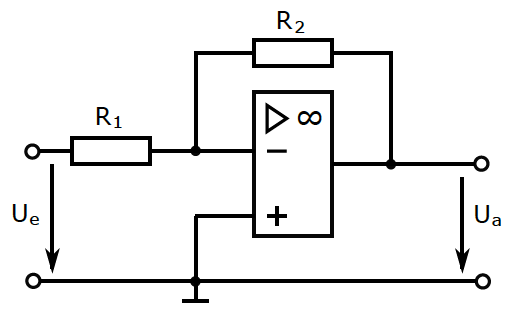
\includegraphics[scale=0.5]{ressources/figure_03.png}
  \caption{Schaltskizze eines invertierenden Linearverstärkers \cite{sample}.}
  \label{fig:03}
\end{figure}
\noindent Eine am invertierenden Verstärker anliegende, positive Eingangsspannung
führt zu einer negativen Ausgangsspannung am Ausgang, welche über den Widerstand
$R_2$ auf den invertierenden Eingang des Operationsverstärkers zurückgeführt
wird und auf diese Weise die Wirkung der positiven Eingangsspannung geschwächt.
Der Liegt keine Eingangsspannung an, ist auch keine Ausgangsspannung oder
Differenzspannung messbar. Wird die Eingangsspannung erhöht, reagiert die Schaltung
auf den Signaleingang. Durch die Spannungsaufteilung auf die in Reihe
geschalteten Widerstände resultiert eine Differenzspannung, welche den
Operationsverstärker an die negative Aussteuerungsgrenze bewegt. Je mehr sich
der Operationsverstärker seiner Aussteuerungsgrenze nähert, desto geringer wird
die Differenzspannung an seinen Eingängen Durch die Gegenkopplung beschränkt sich
der Operationsverstärker in seiner Verstärkungswirkung selbst ab.
Mathematisch beschreiben lassen sich diese Vorgänge unter der Annahme eines
Widerstandsverhältnisses $\frac{R_2}{R_1} << V$ durch
\begin{align}
  I_e = - I_a = \frac{U_e}{R_1} = - \frac{U_a}{R_2} \\
  \implies \frac{U_a}{U_e} = V' = -\frac{R_2}{R_1},
  \label{eqn:05}
\end{align}
\noindent mit $V'$ als Leerlaufverstärkung. Neben der Größe des Eingangssignals
ist auch die Frequenz $\nu$ des Eingangssignals für den Betrieb von
Operationsverstärkern von Bedeutung. Für hohe Frequenzen zeigt sich, dass die
Verstärkung rapide abnimmt. Die Grenzfrequenz ist erreicht, sobald das
Signal auf einen Wert $U_a = \frac{U_e}{\sqrt{2}}$ abgefallen ist \cite{fredenau, sample}.
\subsubsection{Umkehr-Integrator}
\noindent Wird der Widerstand $R_2$ aus \autoref{fig:03} durch einen
Kondensator ersetzt, so ergibt sich die in \autoref{fig:04} dargestellte
Schaltskizze eines Umkehr-Integrators.
\begin{figure}
  \centering
  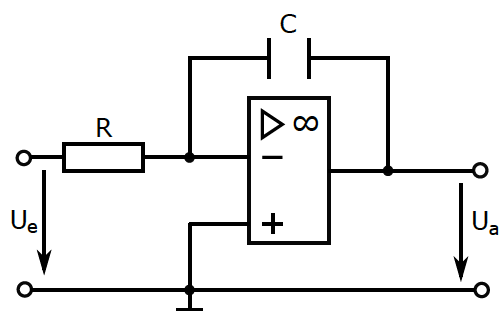
\includegraphics{ressources/figure_04.png}
  \caption{Schaltskizze eines Umkehr-Integrators mit Operationsverstärker \cite{sample}}
  \label{fig:04}
\end{figure}
\noindent Mithilfe von Integratorschaltungen mir eingesetzten
Operationsverstärker lassen sich elektrische Signale integrieren. Dabei gilt die
Beziehung
\begin{align}
  I_1 = \frac{U_e}{R} = - I_2 = - \frac{dQ}{dt} = - C \cdot \frac{d U_A}{dt}.
  \label{eqn:06}
\end{align}
\noindent Für den Anfangswert $U_A(t=0) = 0$ berechnet sich das zugehörige
Integral zu
\begin{align}
  U_A = - \frac{1}{R \cdot C} \cdot \int_0^{t_1} U_E(t) dt
  \label{eqn:07}
\end{align}
\noindent (nach \cite{muenster}).
\subsection{Invertierender Differenzierer}
\noindent Werden bei sonst gleichbleibenden Aufbau die Positionen von Widerstand
und Kondensator getauscht, führt die in \autoref{fig:05} abgebildete Schaltung
die Funktion eines Differenzierers aus. Für die Ausgangsspannung eines
invertierenden Differenzierers gilt die Gleichung
\begin{align}
  U_A = - R \cdot C \cdot \frac{d U_e}{dt}
  \label{eqn:08}
\end{align}
nach \cite{osnabrueck}.
\begin{figure}
  \centering
  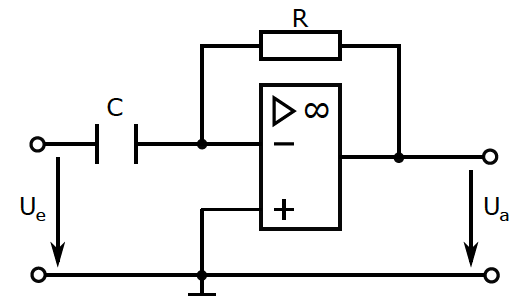
\includegraphics[scale=0.5]{ressources/figure_05.png}
  \caption{Invertierende Differenziererschaltung \cite{sample}.}
  \label{fig:05}
\end{figure}
\subsection{Schmitt-Trigger}
\noindent Im Gegensatz zu den bisher betrachteten Schaltungen mit Gegenkopplung
wird bei der Schmitt-Trigger-Schaltung der zurückgeführte Teil der
Ausgangsspannung auf den nicht-invertierenden Eingang geschaltet. Diese Mitkopplung
zeichnet sich daher durch eine Selbsterhaltung aus: das rückgeführte
Ausgangssignal erhöht das Eingangssignal, es treten Hystereseeffekte in
Erscheinung \cite{elektrotechnik}. Als sogenannter Komparator vergleicht eine
Schmitt-Trigger-Schaltung die Eingangsspannung mit einer Differenzspannung.
Bei Überschreitung der Referenzspannung kippt die Schaltung auf den Wert ihrer
positiven oder negativen Aussteuergrenze.
\begin{figure}
  \centering
  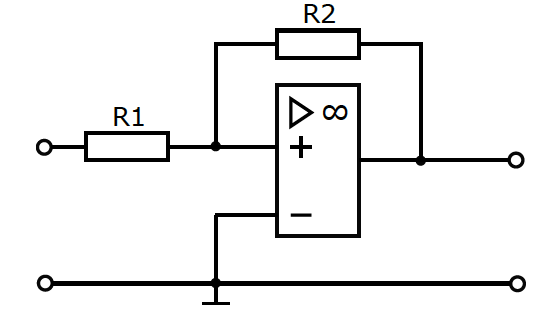
\includegraphics[scale=0.5]{ressources/figure_06.png}
  \caption{Schaltskizze eines Schmitt-Triggers \cite{sample}}
  \label{fig:06}
\end{figure}
\noindent Die Kippspannung des Schmitt-Triggers berechnet sich nach \cite{federau}
über die Relation
\begin{align}
  U_\text{kipp} = U_B \cdot \frac{R_1}{R_P},
  \label{eqn:09}
\end{align}
wobei $R_P$ den Widerstand bezeichnet, über welchen das Signal zurückgeführt
wird. \\
\noindent Eine Schmitt-Trigger-Schaltung mit nachgeschalteten Umkehr-Integrator
lässt sich dazu nutzen, Rechteck- oder Dreieckspannungen zu erzeugen.
Das Kippen der Schmitt-Trigger-Schaltung ist dabei der Auslöser für einen
stetigen Sprung der Ausgangsspannung. Der theoretische Wert der Schwingungsfrequenz
einer Dreieckschaltung berechnet sich nach \cite{sample} über
\begin{align}
  \nu_\text{Dreieck} = \frac{R_2}{4 \cdot C \cdot R_1 \cdot R_3}.
  \label{eqn:10}
\end{align}
\begin{figure}
  \centering
  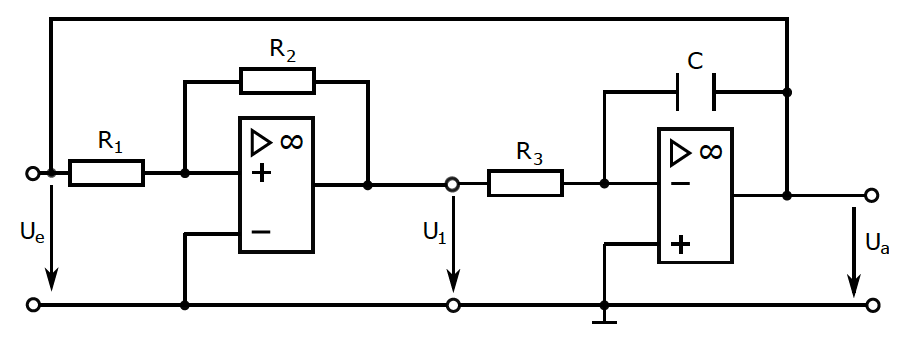
\includegraphics{ressources/figure_07.png}
  \caption{Darstellung einer Schaltung zur Signalgenerierung \cite{sample}.}
  \label{fig:07}
\end{figure}
